% =============================================================================
% Chapitre 6 — Révisions, qualité de mesure et gouvernance de la preuve
% =============================================================================

\chapter{Révisions, qualité de mesure et gouvernance de la preuve}
\label{chap:gouvernance-preuve}

Un projet quantitatif n'est pas crédible parce que son dernier chiffre est
favorable. Il l'est lorsque ce chiffre peut être relié à une source, à une
définition économique, à un protocole temporel et à une version précise du
code. Cette exigence est particulièrement forte dans une banque ou une compagnie
d'assurance : une décision peut être revue longtemps après son émission, par
une seconde ligne de validation, un auditeur ou un régulateur. Il faut alors
reconstituer non seulement le modèle, mais la donnée et les règles qui ont
produit la décision.

Ce chapitre présente une partie moins visible, mais déterminante, du travail :
les corrections qui ont changé le verdict et les contrôles ajoutés pour qu'une
erreur analogue devienne détectable automatiquement. Il ne s'agit pas d'un
journal d'incidents. C'est la démonstration que le prototype sait retirer une
conclusion lorsque ses hypothèses ne tiennent plus.

% -----------------------------------------------------------------------------
\section{Trois mesures du même système, trois verdicts}
% -----------------------------------------------------------------------------

La figure~\ref{fig:revision-resultat} résume l'évolution du résultat principal
sur \texttt{full\_2021}. Les deux premiers nombres sont conservés comme
\textbf{résultats historiques superseded}, et non comme performances actuelles.

\begin{figure}[htbp]
  \centering
  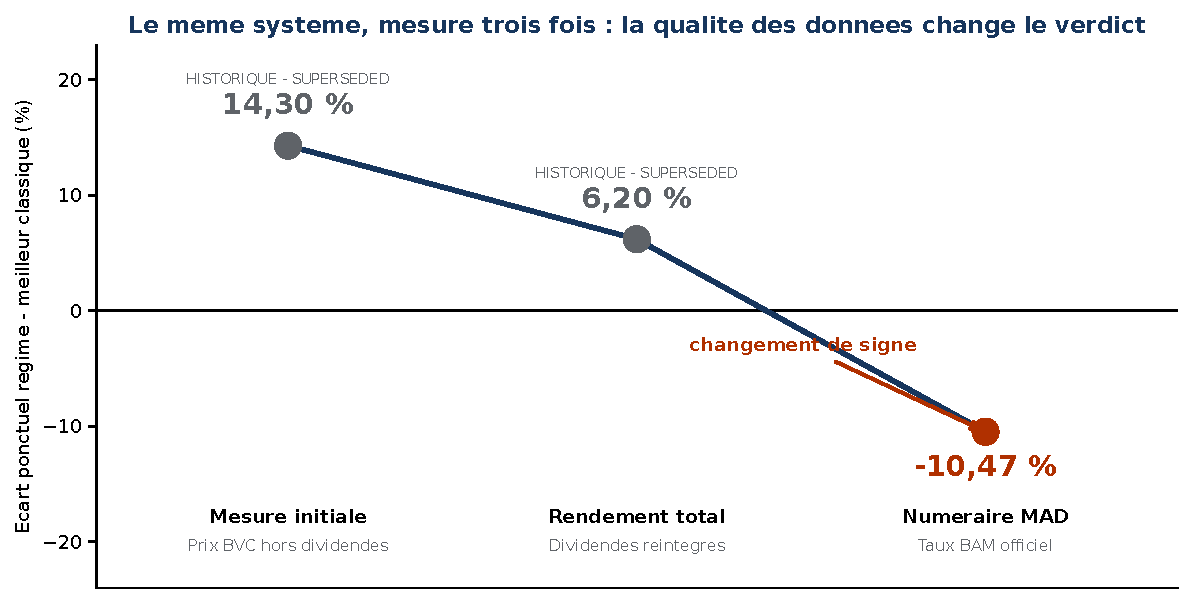
\includegraphics[width=0.96\textwidth]{assets/figures/revisions_resultat.pdf}
  \caption{Évolution du résultat après correction successive de la définition
  du rendement et du numéraire. Les deux valeurs positives sont historiques et
  remplacées par la mesure en MAD. Source : artefacts Gold versionnés.}
  \label{fig:revision-resultat}
\end{figure}

\paragraph{Mesure initiale.} Les ETF étaient fournis en rendement total, tandis
que les actions de la Bourse de Casablanca étaient observées en prix seulement.
La comparaison attribuait donc aux optimiseurs le mérite d'éviter des actifs
dont une partie du rendement avait été supprimée par la préparation des
données. La réintégration causale des dividendes aux dates de détachement a
réduit l'écart observé de $+14{,}3$~\% à $+6{,}2$~\%.

\paragraph{Correction du numéraire.} Cette seconde correction est plus
fondamentale. Un rendement est un ratio sans unité, mais un portefeuille produit
un profit ou une perte dans une devise. Additionner quatre rendements en MAD et
cinq rendements en USD sans conversion revient à agréger des montants qui ne
sont pas réalisables par un même investisseur. Après conversion causale des
niveaux de prix ETF au taux de référence USD/MAD de Bank Al-Maghrib, l'écart
ponctuel devient $-10{,}47$~\% : 0,9571 de Sharpe net pour
\texttt{regime\_conditional}, contre 1,0690 pour \texttt{max\_sharpe}.

\begin{resultatbox}{La contribution n'est pas le changement de signe}
Le point important n'est pas que le résultat soit devenu défavorable au ML. Il
est que l'architecture ait permis de localiser l'hypothèse économique erronée,
de reconstruire toute la chaîne avec la source officielle, puis de retirer le
message antérieur sur chaque surface publiée. Un résultat qui résiste à une
tentative de réfutation vaut davantage qu'un résultat favorable obtenu une fois.
\end{resultatbox}

% -----------------------------------------------------------------------------
\section{Le numéraire : une notion simple aux conséquences matérielles}
% -----------------------------------------------------------------------------

Le \emph{numéraire} est la monnaie dans laquelle le patrimoine et sa performance
sont mesurés. Pour un investisseur marocain, acheter un ETF américain crée deux
sources de variation : celle de l'ETF en dollars et celle du dollar face au
dirham. En l'absence de couverture, les deux appartiennent au rendement réalisé.

\begin{figure}[htbp]
  \centering
  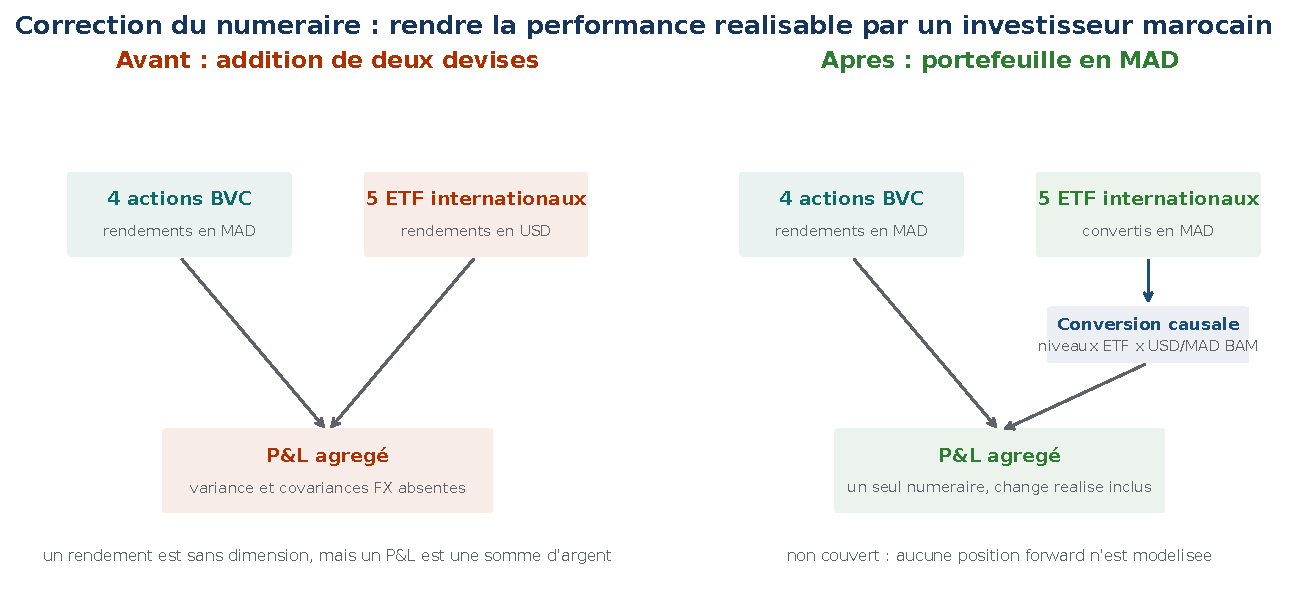
\includegraphics[width=\textwidth]{assets/figures/numeraire.pdf}
  \caption{Avant et après correction du numéraire sur l'univers mixte. La
  conversion est appliquée aux niveaux de prix avec uniquement l'information
  disponible à la date considérée ; aucune position de couverture n'est simulée.}
  \label{fig:numeraire}
\end{figure}

La politique finale est donc définie \emph{par univers}, sans valeur globale par
défaut :

\begin{itemize}
  \item \texttt{full\_2021} contient quatre actions BVC et cinq ETF. Il est
        entièrement exprimé en \textbf{MAD}, au taux officiel BAM, et reste
        \textbf{non couvert} contre le risque USD/MAD ;
  \item \texttt{etf\_2017} contient uniquement cinq ETF en USD. Il reste un
        univers \textbf{USD mono-devise}, indépendant de la série BAM ;
  \item les deux univers répondent à des questions différentes. Leurs niveaux
        de Sharpe ne doivent pas être comparés entre eux comme s'ils partageaient
        le même investisseur de référence.
\end{itemize}

La source Yahoo initialement envisagée a été refusée par un contrôle de qualité :
sur les dates communes, elle suivait le niveau du taux de change, mais ses
variations quotidiennes étaient presque décorrélées de celles de BAM et sa
volatilité était environ six fois plus élevée. La série officielle couvre
entièrement la période exploitable de \texttt{full\_2021}. Une lacune initiale
de dix-sept jours ouvrés a conduit à déplacer le début de l'univers au 29 juillet
2021 ; la fenêtre hors échantillon publiée n'est pas affectée.

% -----------------------------------------------------------------------------
\section{Le protocole fait partie du résultat}
% -----------------------------------------------------------------------------

Deux expériences honnêtes peuvent aboutir à un classement différent si elles
n'interrogent pas la même période. La figure~\ref{fig:protocoles} distingue le
découpage unique de la phase~5 du \emph{walk-forward} imbriqué. Dans les deux
cas, l'entraînement reste strictement antérieur à l'évaluation. Dans le second,
la sélection est répétée à chaque frontière externe, ce qui change aussi la
fenêtre hors échantillon concaténée.

\begin{figure}[htbp]
  \centering
  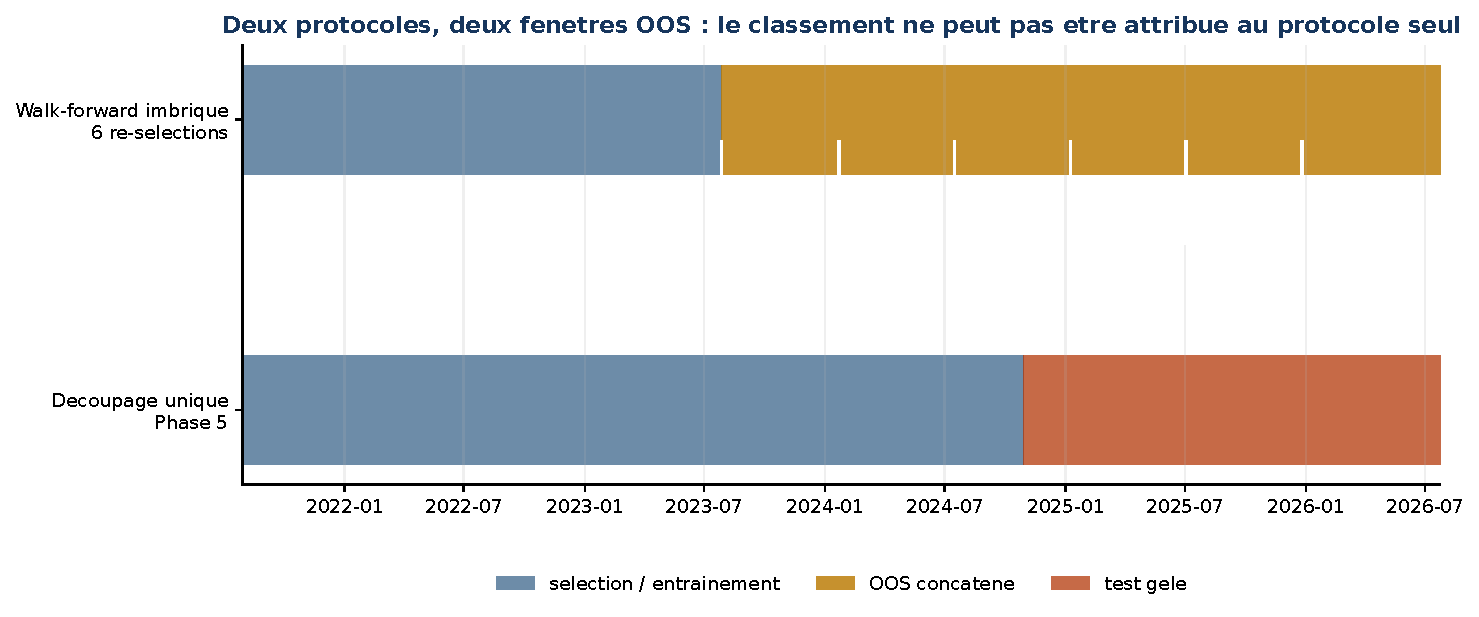
\includegraphics[width=0.98\textwidth]{assets/figures/protocoles.pdf}
  \caption{Protocoles temporels comparés. Une purge retire les observations
  dont l'horizon de cible chevauche la validation ; l'embargo impose un espace
  supplémentaire à la frontière.}
  \label{fig:protocoles}
\end{figure}

Sur la fenêtre imbriquée du 28 juillet 2023 au 24 juillet 2026, six
re-sélections produisent 781 observations hors échantillon. Le ratio de Sharpe
déflaté est 0,6707 sur 198 configurations. Aucun adjectif n'est accolé à cette
valeur : aucun seuil d'interprétation n'a été fixé avant l'expérience. La
conclusion défendable est plus sobre : \textbf{le classement est sensible au
protocole et à la fenêtre hors échantillon associée}. Il serait incorrect
d'attribuer la différence au seul caractère imbriqué du protocole.

% -----------------------------------------------------------------------------
\section{Du data snooping à une conclusion corrigée}
% -----------------------------------------------------------------------------

Choisir le meilleur résultat parmi de nombreuses configurations augmente
mécaniquement la probabilité de trouver une performance apparente. Ce phénomène,
appelé \emph{data snooping}, est l'équivalent quantitatif de poser 240 questions
au même échantillon puis de ne rapporter que la réponse la plus favorable.

\begin{figure}[htbp]
  \centering
  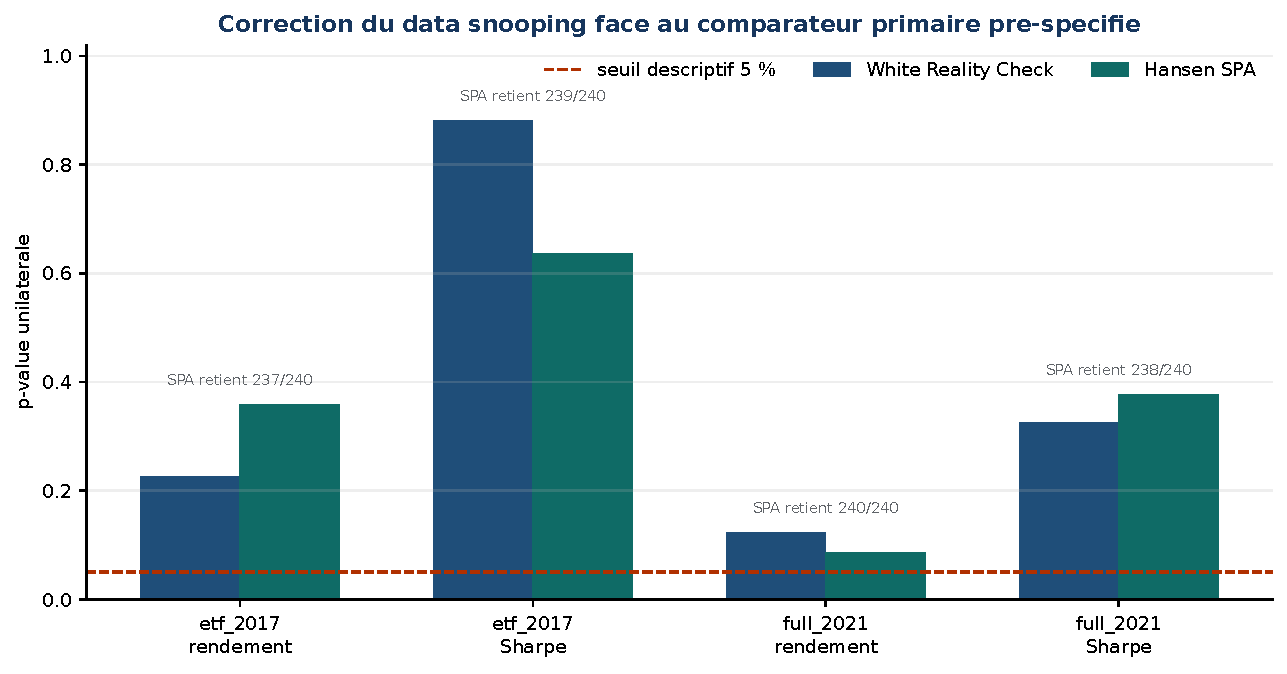
\includegraphics[width=0.95\textwidth]{assets/figures/multiple_testing.pdf}
  \caption[Correction White/SPA sur 240 configurations]{White Reality Check et Hansen SPA face au comparateur primaire
  \texttt{regime\_conditional}. Aucun des quatre tests primaires ne franchit le
  seuil descriptif de 5~\%. Les deux procédures sont toujours publiées ensemble.}
  \label{fig:multiple-testing-final}
\end{figure}

Le comparateur primaire \texttt{regime\_conditional} a été fixé avant lecture
des valeurs corrigées et n'a pas été remplacé après le changement de signe. Sur
240 configurations atteignables, aucun candidat n'établit une surperformance
contre ce comparateur, sur aucun univers et pour aucune des deux statistiques
évaluées. Les comparaisons à l'équipondéré sont conservées comme exploratoires :
franchir ce plancher ne prouve pas que la couche ML apporte une valeur
incrémentale.

Cette correction ne se substitue pas au bootstrap pairé. Les deux répondent à
des questions différentes : le bootstrap teste la différence entre deux séries
alignées sur les mêmes jours ; White/SPA corrige le fait que de nombreux
candidats ont été essayés. Par ailleurs, l'absence de rejet ne démontre jamais
l'équivalence. Un test d'équivalence exigerait une marge économique définie à
l'avance.

% -----------------------------------------------------------------------------
\section{Une chaîne de preuve exécutable}
% -----------------------------------------------------------------------------

La succession des corrections a conduit à une règle de conception : une
affirmation critique ne doit pas dépendre de la mémoire de l'équipe. Elle doit
être liée à un contrôle qui échoue si l'affirmation devient fausse.

\begin{figure}[htbp]
  \centering
  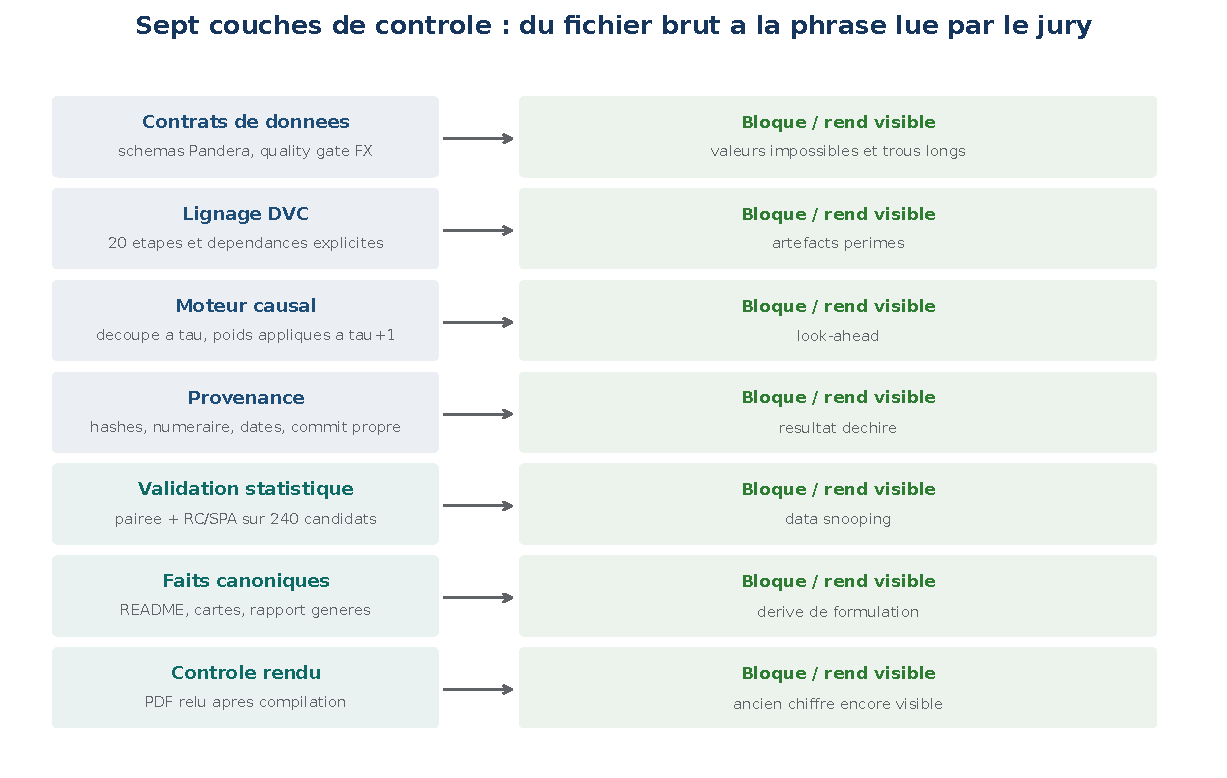
\includegraphics[width=0.98\textwidth]{assets/figures/chaine_preuve.pdf}
  \caption{Sept couches de contrôle entre la donnée et la phrase publiée. Chaque
  garde-fou est né d'une classe d'erreur effectivement observée dans le projet.}
  \label{fig:chaine-preuve}
\end{figure}

Les contrats Pandera bloquent les valeurs impossibles et les trous trop longs.
DVC relie chaque produit à ses dépendances et rend le graphe reconstruisible.
Le moteur causal tronque toutes les données à la date de décision. Le manifeste
de snapshot enregistre les empreintes, le numéraire, les dates et la révision
productrice ; il refuse de certifier un arbre Git non propre. Les tests
statistiques conservent les séries pairées et le nombre de candidats. Enfin, les
faits publiés sont générés depuis Gold puis vérifiés jusque dans le texte extrait
du PDF. Ce dernier contrôle a détecté des valeurs historiques que les recherches
dans le code source avaient manquées à cause de la syntaxe LaTeX.

\begin{remarquebox}
L'auditabilité n'est pas synonyme d'immuabilité du résultat. Au contraire, un
système gouverné doit pouvoir changer de conclusion lorsque la donnée ou le
protocole change, tout en expliquant exactement pourquoi et à partir de quelle
version.
\end{remarquebox}

% -----------------------------------------------------------------------------
\section{Intégrité des modèles sous défaillance}
% -----------------------------------------------------------------------------

Les estimateurs DCC--GARCH et les modèles de rendement possèdent des chemins de
repli sûrs. Sans télémétrie, un résultat intitulé « DCC--GARCH » pourrait en
réalité être produit par Ledoit--Wolf après une non-convergence. Chaque
rééquilibrage enregistre donc le modèle demandé, le modèle effectif, le statut,
la raison du repli, le nombre de lignes d'entraînement et les avertissements de
convergence.

Sur le snapshot publié, 0 des 1\,188 ajustements — quatre stratégies et 297
dates de rééquilibrage sur les deux univers — ont utilisé un repli. Cela ne
signifie pas qu'un modèle ne peut jamais échouer : les chemins sont testés et un
autre snapshot peut les activer. Cela établit seulement, mais précisément, que
chaque performance publiée sur cette version provient du modèle indiqué par son
étiquette. Les caches réémettent la télémétrie à chaque lecture, afin qu'un cache
chaud ne fasse pas artificiellement diminuer le taux de repli.

% -----------------------------------------------------------------------------
\section{Lecture pour une organisation financière régulée}
% -----------------------------------------------------------------------------

Dans un environnement bancaire ou assurantiel, cette architecture prépare trois
niveaux de contrôle usuels. La première ligne — l'équipe qui construit — produit
les artefacts, tests et cartes de modèle. Une seconde ligne indépendante devrait
challenger les données, hypothèses de coûts, décisions de modèle et seuils. Une
troisième ligne d'audit doit pouvoir rejouer ou retracer la release sans dépendre
des auteurs. Le projet livre la matière technique des trois niveaux, mais ne
prétend pas avoir réalisé la validation indépendante : cette case reste
explicitement ouverte dans la gouvernance.

Le prototype est donc \textbf{documenté et reproductible}, pas « validé pour la
production ». Cette distinction est importante : elle évite qu'une qualité
d'ingénierie réelle soit transformée en autorisation d'usage que le projet n'a
ni le mandat ni les données pour accorder.
